\section{Desgin}

The PUSH shell is a conventional UNIX shell with 
two additional pipeline operators, a multiplexing 
fan-out(\verb!|<![\emph{n}]), and a coalescing fan-in(\verb!>|!).
This combination allows PUSH to distribute I/O to and from multiple
simultaneous threads of control.
A fan-out argument, \emph{n}, specifies the desired degree of parallel
threading.  If no argument is specified, the default of spawning a new
thread per record (up to the limit of available cores) is used.  This can
also be overriden by command line options or environment variables.
The pipeline operators provide implicit grouping semantics allowing natural
nesting and composibility.
While their complimentary nature usually lead to symmetric
mappings (where the number of fan-outs equal the number of fan-ins), there is
nothing within our implementation which enforces it.
Normal redirections as well as application specific sources and sinks
can provide alternate data paths.

\begin{figure}[htp]
\centering
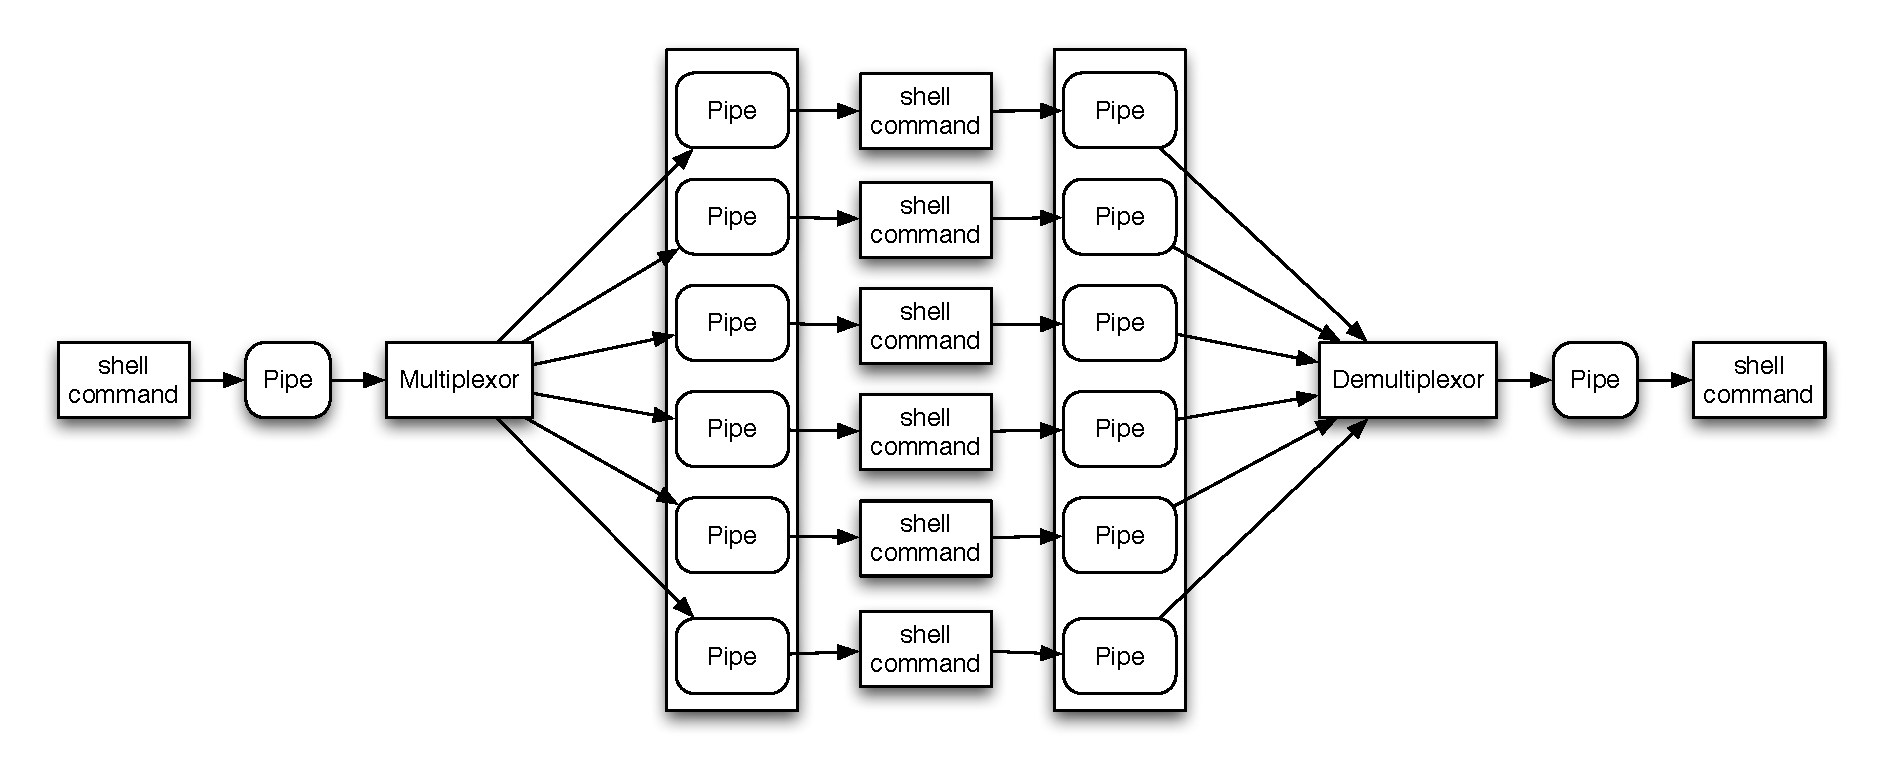
\includegraphics[width=3in]{pipestruct.eps}
\caption{The structure of the PUSH shell}
\label{fig:pipestruct}
\end{figure}

PUSH also differs from traditional shells by implementing native support for
record based input handling over pipelines. This facility is similar to the
argument field separators, IFS and OFS, in traditional shells which use a
pattern to determine how to tokenize arguments. PUSH provides two variables,
ORS and IRS, which point to record separator modules. These modules
(called multiplexors in PUSH) split data on record boundaries, emitting
individual records that the system distributes and coalesces.
The choice of which \emph{multipipe}, an ordered set of pipes, to target is
left as a decision to the module.

Different data formats may have different output requirements.  
Demultiplexing from a multipipe is performed by creating a many to one
communications channel within the shell. The shell creates a reader processes
which connects to each pipe in the multipipe. When the data reaches an
appropriate record boundary a buffer is passed from the reader to the shell
which then writes each record buffer to the output pipeline.

% EVH: the example here may be superfluous as its really just justifying
% map/reduce, not the particulars of the PUSH implementation.
An example from our particular experience, Natural Language Processing, is
to apply an analyzer to a large set of files, a "corpus". User programs go
through each file which contain a list of sentences, one sentence per line.
They then tokenize the sentence into words, finding the part of speech and
morphology of the words that make up the sentence.
There are a large number of discrete sets of data whose order is not 
necessarily important. We need to perform a computationally intensive task 
on each of the sentences, which are small, discrete records an ideal target 
for parallelization.

PUSH was designed to exploit this mapping. For example, to get a histogram of
the distribution of Japanese words from a set of documents using chasen,
a Japanese morphological analyzer, we take a set of files containing sentences
and then distribute them to a cluster of machines on our network. The command
is as follows:
%
% This example is horribly complex, I favor a more simple formulation
% even if its faked a bit
%
%push -c '{
%  ORS=./blm.dis  du -an files |< xargs os \\
%   chasen | awk '{print \$1}' | sort | uniq -c \\
%   >| sort -rn
%}'
\begin{verbatim}
    ORS=blm find . -type f |< \\
    xargs chasen | sort | uniq -c >| sort -rn
\end{verbatim}

The first variable, ORS, declares our record multiplexor module, 
the intermediary used to ensure that the input and output to 
distributed pipes are correctly aligned to record boundaries. 
In many cases a default which splits based on atomic writes can
be used.  Alternatively one of several built-ins which split based on 
a field separator or newline can be used.

\emph{find . -type f} gives a list of the files
which are then "fanned out"(\verb!|<!) using a combination
of a multipipes, and a \emph{multiplexor}
which determines which pipes are the targets of each unit of output.
This fanned out data goes to xargs on new threads
which then uses the filenames as arguments to
chasen. The find acts as a command driver, fanning out file names to the
individual worker machines. The workers then use the filenames input to
xargs, which uses the input filenames as arguments to the target command.
Using the output of the analyzer (Japanese words) are then sorted and 
counted using uniq.  Finally these word counts are "fanned in"(\verb!>|!) 
to the originating machine which then sorts them.

While PUSH works perfectly well on a stand-alone machine, the original
intent was to use it to drive workloads and workflows across a cluster of
machines.  In particular, we were interested on deploying on leadership
class high performance computing machines and as such
a key requirement for us was scalability to a large number of nodes.  
Instead of traditional client/server models we opted for a peer based
model where every node within the system is capable of initiating new
workflows of computation and managing the newly created pipeline.
This allows workflows and component applications to initiate new branches
of computation or analysis at any stage of the pipeline or in reaction to
data produced by a previous portion of the pipeline giving the entire
infrastructure a degree of elasticity that seemed to missing from 
previously available tools.
In order to accomplish this we designed the system without any central
component which required knowledge of the entire system.
All knowledge is distributed and then aggregated at certain points.
Descisions like scheduling and job management are also made in a
distributed fashion, utilizing the hierarchy of aggregation points
to eliminate the need for all-to-all communication during workload
distribution.

In order to scale such a system we decided to go with a hierarchical
organization of nodes.  
Aggregation points scale command and communication between nodes.  
When a node or its children have insufficient resources to satisfy a request,
the request is propagated to the parent aggregation point.
This form of hierarchical aggregation also seems to map well with the 
physical topology of many leadership class systems.
The hierarchical topology not only helps scale communication and control,
but it also can help users and application components traverse multiple
network domains in a seamless fashion.
We intend to use this property to create an environment which seamlessly
extends the user's desktop experience and environment to the supercomputer.

The forms of communication aggregation match the new pipeline primatives 
which are part of the PUSH shell.
By default, input to each master pipeline component thread is fanned out 
to sub-session threads and output from those sub-sessions in fanned back
into the master component.
It is intended that this behavior be setup and controlled by the XCPU
infrastructure which spawns the sub-session threads (whether they be local
or remote).
For multi-stage pipelines, we need the ability to direct the output of
a pipeline component to another pipeline component without necessarily
passing that data through the master thread (for efficiency reasons).
In order to accomplish that we've added the ability to splice input or
output of individual subsessions threads to eachother.
